\subsection{Air Traffic Management (ATM)}

\Gls{ATM} is the aggregation of the airborne and ground-based functions required to ensure the safe and efficient movement of aircraft during all phases of operations, through controlled airspaces and on the ground at airports \cite{skybraryATM}.
It comprises serveral components, including \gls{ATS}, \gls{ASM}, and \gls{ATFM} \cite{skybraryATM}.
Figure \ref{fig:atm-structure} shows the structure of \gls{ATM} and the relationship between \gls{ATS}, \gls{ASM}, and \gls{ATFM}.

\begin{figure}[h]
    \centering
    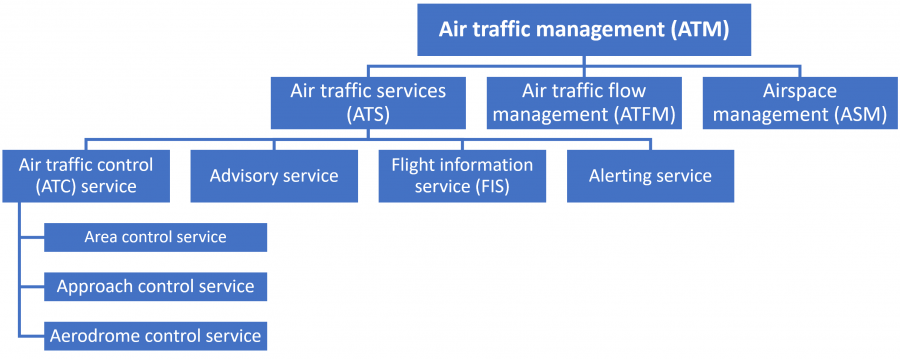
\includegraphics[width=0.8\linewidth]{900px-ATM_Chart.png}
    \caption{Structure of \gls{ATM} \cite{skybraryATM}}
    \label{fig:atm-structure}
\end{figure}

\Glspl{ATCO}, part of \gls{ATC} service, are responsible for directing aircraft safely and efficiently, managing takeoffs and landings, maintaining safe distances between aircraft en route and handling emergencies. 
Their role demands high levels of situational awareness, rapid decision-making, and the ability to manage multiple tasks under high stress conditions.
These indispensable skills, such as judgement, flexibility and the ability to handle unexpected situations, remains critical and are not easily replicated by automated systems \cite{eurocontrol2024digitalisation}.